\textbf{Uiteindelijk richt het managementteam de organisatie in en is verantwoordelijk voor alles dat in de onderneming om gaat. Het is dan niet verbazingwekkend dat leidinggevenden en strategiemakers een sterke behoefte hebben aan frequent, kwalitatief, en relevante managementinformatie. Hand-in hand hiermee gaat het middel waardoor de boodschap wordt overgedragen: communicatie. In dit hoofdstuk wordt gekeken welke informatie in de organisatie beschikbaar is en hoe deze gepresenteerd wordt.}

\begin{table}[!h]
    \centering
    \caption{Excerpt van de principes voor interne controle volgens COSO}
    \begin{tabular}{l l}
        \toprule
        \textbf{Element} & \textbf{Principe} \\
        \midrule
        Informatie en communicatie & 13. Gebruikt relevante en kwalitatieve \\
        & informatie om de interne controle te handhaven \\
         & 14. Geeft intern de interne controle \\
         & informatie te kennen \\
         & 15. Geeft extern de interne controle \\
         & informatie te kennen \\
        \bottomrule
    \end{tabular}
    \label{tab:informatieprincipes}
\end{table}

In het COSO-raamwerk valt SFC onder het dertiende en het vijftiende principe. Deze zijn gekozen doordat SFC niet alleen intern een behoefte heeft aan frequent overleg om de verkoopplannen af te stemmen, ook is er een belangrijke compliance rol die vervult moet worden richting het Japanse moederbedrijf. 

Intern is er dagelijks overleg tussen de afdelingen. Niet al deze besprekingen worden formeel vastgelegd, wel heeft dit tot gevolg dat problemen makkelijk bespreekbaar zijn en dat samenwerking bevorderd wordt. Er zijn een aantal besprekingen die wél formeel geregeld zijn. Deze zijn in figuur \ref{fig:overleg2} weergegeven. 

\newpage

\begin{figure}[h!]
    \centering
    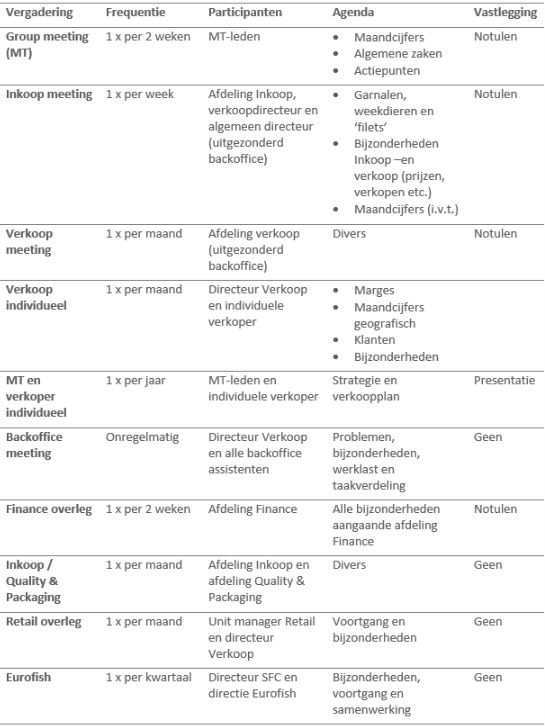
\includegraphics[width=1\textwidth]{overleg}
    \caption{Overlegstructuur SFC \citep{aoibsfc}}
    \label{fig:overleg2}
\end{figure}

\newpage 
Door de introductie van Exact Synergy is het mogelijk om de \gls{geldgoederen} veel nauwkeuriger te volgen. Voor elke stap in het proces zijn de medewerkers in staat om containers en verschepingen te tracken. Niet alleen stelt dit de afdelingen in staat om een vloeiende samenwerking te oriënteren tussen de afdelingen, ook is het mogelijk om de klant te informeren over de status en de verschepingsdetails. Het stelt de registrerende en controlerende medewerkers in staat om extra verband- en detailcontroles uit te voeren, en het managementteam kan conclusies trekken over omlooptijd en andere details over gehele perioden. \citep{aoibsfc}

In relatie tot begroting, vorige perioden, en productcategorie:
\begin{itemize}
    \item Exploitatie: \\
    Omzet \\
    \underline{-/- Kostprijs verkopen} \\
    Brutomarge \\
    -/- Verkoopkosten \\
    \underline{-/- Apparaatkosten} \\
    Nettomarge \\
    \item Balans gerelateerd: \\
    Omloopsnelheid van de voorraad \\
    Ouderdom van de openstaande debiteuren \\
    Openstaande crediteuren \\
    Voorraadverschillen \\
    Solvabiliteitsratio's \\
    Percentage bederf
\end{itemize}

Er zijn bij SFC een aantal expat medewerkers in dienst die namens Maruha Nichiro onder andere rapportage en compliance verzorgen naar het moederbedrijf. Hiervoor gaan zij gesprekken aan en stellen zij vragen aan de desbetreffende medewerkers. Deze vragen komen vanuit Maruha Nichiro en wordt beantwoord door rapportage terug naar Japan door de expats. De informatievoorziening is hier dus minder kwantitatief van aard en is juist meer gericht op de systemen en processen.

\subsection*{Conclusie}
De beschikbare informatie is drastisch toegenomen door de introductie van Exact Synergy. Niet alleen is het nu overzichtelijker voor medewerkers om inzicht te krijgen in het proces, ook is het voor toezichthoudende en controlerende personen eenvoudiger gemaakt om uitgebreide rapportage op te stellen. Externe informatieverschaffing gaat echter niet kwantitatief, maar door werkzame expats bij SFC. Het is relatief eenvoudig om kengetallen te genereren waarmee de betrouwbaarheidsrisico's geanalyseerd kunnen worden.


\begin{comment}
\textbf{Concrete vragen}
\begin{itemize}
    \item Welke informatie is voorhanden aan directie over belangrijke betrouwbaarheids- en bedrijfsrisico's?
    \item Wat is de kwaliteit van de communicatie binnen de organisatie?
    \item Wat is de kwaliteit van de communicatiesystemen binnen de organisatie?
    \item Wordt er voldaan aan de compliance voor externe verslaggeving? 
    %Volgen van NL-GAAP in de externe jaarrekening met betrekking tot verwerking in te kopen / ingekochte vreemde valuta. Wordt nu verwerkt als \textit{niet uit de balans blijkende verplichtingen}, maar er hangt natuurlijk ook een niet uit de balans blijkend recht aan
\end{itemize}
\end{comment}

\newpage